\begin{frame}{Task flow LU ($A = LU$)}
In order to cope with the task flow model, linear algebra algorithms are expressed in terms of tasks operating on fine grain squares sub-matrices, also called tiles.
\begin{columns}
\begin{column}{0.02\textwidth}
\end{column}
\begin{column}{0.5\textwidth}
\begin{overprint}
\includegraphics<1>[width=0.9\linewidth]{free}
\includegraphics<2>[width=0.8\linewidth]{free_tiled}
\includegraphics<3>[width=0.8\linewidth]{task_getrf}
%\includegraphics<4>[width=0.8\linewidth]{task_trsm_l}
\includegraphics<4>[width=0.8\linewidth]{task_trsm_u}
\includegraphics<5>[width=0.8\linewidth]{task_gemm}
%\includegraphics<7>[width=\linewidth]{dag_getrf_sp}
\includegraphics<6>[scale=0.3]{step_lu}
\end{overprint}
\end{column}
\begin{column}{0.45\textwidth}
\begin{overprint}
\includegraphics<3>[width=0.8\linewidth]{getrf_getrf}
%\includegraphics<4>[width=0.8\linewidth]{getrf_trsm_l}
\includegraphics<4>[width=0.8\linewidth]{getrf_trsm_u}
\includegraphics<5>[width=0.8\linewidth]{getrf_gemm}
\includegraphics<6>[width=0.8\linewidth]{getrf}
\end{overprint}
\end{column}
\end{columns}
\begin{flushleft}
\onslide*<2>{Tiles are not contiguous in memory}
\onslide*<3>{Task to factorize diagonal tiles: GETRF}
\onslide*<4>{Task to update other panel tiles and block line tiles: TRSM\_L and TRSM\_U}
\onslide*<5>{Task to update trailing sub-matrix: GEMM}
\end{flushleft}
\end{frame}

%\begin{frame}{Task Flow LU}
%\framesubtitle{Example on matrix of 3*3 tiles}
%\begin{columns}
%\begin{column}{0.02\textwidth}
%\end{column}
%\begin{column}{0.3\textwidth}
%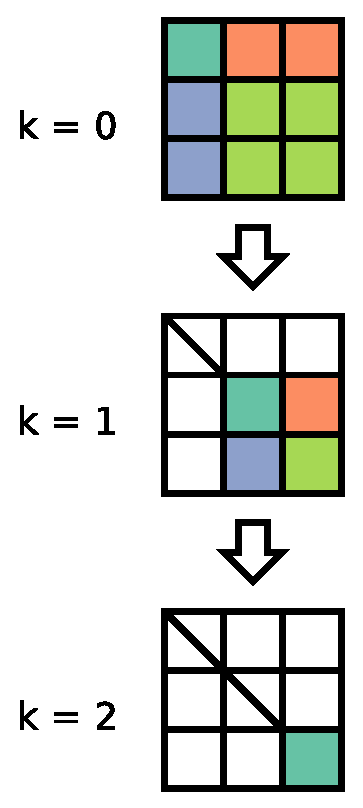
\includegraphics[scale=0.5]{step_lu}
%\end{column}
%\begin{column}{0.6\textwidth}
%\includegraphics[width=\linewidth]{getrf}
%\end{column}
%\end{columns}
%\end{frame}